\documentclass[notitlepage, 10pt, twocolumn]{report} % article also possible. ignored twocolumn option
\usepackage[margin=1.3in]{geometry}
\usepackage{caption}

\usepackage[utf8]{inputenc}
\usepackage[font=small,labelfont=bf]{caption} % caption stuff

\usepackage[]{algorithm2e}
\usepackage{algorithmic}
\usepackage{listings}

\usepackage{lipsum}
\usepackage{titling}

% \usepackage[demo]{graphicx} % [demo] option for empty figure
\usepackage{dblfloatfix}    % To enable figures at the bottom of page

\usepackage{graphicx}
\graphicspath{{./images/}}
\usepackage{amssymb}
\usepackage[T1]{fontenc} % for < and >


\usepackage{titlesec}
\titleformat{\section}
  {\large\bf\scshape}{\thesection}{2em}{}
\titleformat{\subsection}
  {\rm\scshape}{\thesubsection}{0em}{}

% I have no idea what this is tho
\pretitle{\begin{center}\Huge\bfseries}
\posttitle{\par\end{center}\vskip 0.5em}
\preauthor{\begin{center}\large\bfseries}
\postauthor{\end{center}}
\predate{\par\large\centering}
\postdate{\par}

\let\endtitlepage\relax


\title{Solving nonograms using \texttt{A*-GAC}}
\author{Mikael Kvalvær}
\date{\today}

% \begin{abstract}
%   


% \end{abstract}
% \maketitle

\begin{document}
\maketitle

\section{Representation of the problem}
  \newenvironment{myitemize} % hacks
{ \begin{itemize}
    \setlength{\itemsep}{0pt}
    \setlength{\parskip}{0pt}
    \setlength{\parsep}{0pt}     }
{ \end{itemize}                  } 

An aggregate representation was used for this project. Aggregate representation
looks at rows and columns as the fundamental units. The preprocessing takes
somewhat more time, but the advantage is good computational performance and
simpler code. Next follows a short description of the variables, domains and
constraints employed in the representation.\\

\begin{figure}[b]
    \centering
    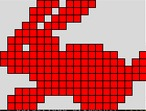
\includegraphics[width=0.25\textwidth]{rabbit.jpg}
    \caption{Example of a solved nonogram-puzzle. The red boxes marks cells
    that are common for both column and row.} 
    
\end{figure}

\noindent
\textbf{variables}: Consider the figure of the rabbit. The first row consists of the feet of the rabbit, where the feet touches the ground.
The segment lengths are 4 and 5. The variable here is defined as the entries in the row.
Therefore, we have a single variable for the first row, with the value $[0, 1, 1, 1, 1, 0, 0, 0, 0, 0, 0, 1, 1, 1, 1, 1, 0, 0, 0, 0]$.

In general, we have rows with dimensionality $M$ and columns with dimensionality $N$. Thus, a variable for a row is a vector
$x \in \{0, 1\}^M$ and for a column a vector $y \in \{0, 1\}^N$.\\

\noindent
\textbf{domains}: For each variable $x$ the domain $\mathcal{D}(x)$ is
defined as all feasible values for the variable.  Consider a column with length
$N$ and with $n$ segments, each with length $l_1,\ldots, l_n$. The total
length is $L = \sum_i^N l_i$. For the first segment, the first index the first
cell can be placed is 0.  The last index is found by $M - (n-1) - L$ because the
expression $L + (n-1)$ represent the minimum space occupied by all cells.
For example, we can see in the first row that $M = 20$, $L = 4 + 5 = 9$ and $n-1 = 1$.
From this we can deduce that the last index that the first segment can start on
is $20 - 9 - 1 = 10$. A recursive procedure is applied that finds the domains
for each variable.\\

\noindent
\textbf{constraints}: The discussion above showed how the domains of each
variable is found. We can restrict the domain size by enforcing the domain
size for each row and column.  This will generate a list of possible rows for
each row and a list of possible columns for each column.

Furthermore, each column and row must agree with each other on which cells are marked
and which are not. Any row that marks a cell that is for certain not in the
corresponding column must be removed. Similarly, any column that marks a cell
that is for certain not in the corresponding row must be removed.\\

% \begin{algorithm}
%     \begin{small}
%         \begin{lstlisting}[language=Python, caption=Generation of row / column segments]
% def generate_segments(seg_lengths, tot_length,
%                       min_idx=0,  index=0,
%                       segment=None):
% 
%   if index == 0:  # we're in the base case -- make an empty line
%     segment = np.zeros(tot_length, dtype=np.int64)
% 
%   n_remaining = len(seq_lengths[index:])
%   length_ahead = seg_lengths[index:].sum() + (n_remaining - 1)
% 
%   max_idx = tot_length - length_ahead
% 
%   # place current segment on all possible places
%   for i in range(min_idx, max_idx + 1):
%    new_segment = copy.deepcopy(segment)
%    new_segment[i:i + seg_lengths[index]] = np.int64(1)
%    min_idx_prime = i + seg_lengths[index] + 1
% 
%   is_last_index = index == len(seg_lengths) - 1
%    if is_last_index:  # finished
%      yield new_segment
% 
%    else:  # fix the segment and find remaining possible domains
%      for each in generate_segments(seg_lengths, tot_length,
%                                    min_idx_prime, index+1, new_segment):
%        yield each
% 
%         \end{lstlisting}
%     \end{small}
% \end{algorithm}
% 
% \begin{algorithm}
%     \begin{small}
%         \begin{lstlisting}[language=Python, caption=Filtering of rows (columns) based on entries in columns (rows)]
%         function filter_X_on_Y(X, Y):
%           for y in Y:
%             common_cells = find_common_cells(y)
%             X = remove_x_where_not_present(common_cells)
%           return X
%         \end{lstlisting}
%     \end{small}
% \end{algorithm}
% 
% ..
% 


\section{Heuristics used}
  \subsection*{choice of \texttt{h} function}
A state consists of candidates for each row and column. Let $nc_i$ be the
number of column candidates for column $i$. Similarly, we define $nr_j$ as the
number of candidate rows for row $j$. Then, $h$ is defined as

\begin{displaymath}
  h = \sum\limits_{i \in \texttt{cols}} log(nc_i) + \sum\limits_{j \in \texttt{rows}} log(nr_j)
\end{displaymath}

Logarithm's are used to prevent numerical overflow. This could occur if there
are a large number of rows / columns or if the range is sufficiently large. If any
$nc_i = 1$ then they will not contribute to the heuristic function because $log(1) = 0$.

\subsection*{Choice of variable on next assumption}
The choice of variable on which to base the next assumption is solely based
on the number of candidates (domain cardinality) for that variable. If there
are few candidates, then it will be faster to visit all possible states by
assuming specific values for that variable. On the other hand, if the domain
is large, it'll take more time to visit all subsequent nodes. Therefore, the
line with fewest candidates (greater than 1) is chosen. The algorithm below
implements this and returns the line index with smallest domain.

\begin{algorithm}
\begin{footnotesize}
\begin{lstlisting}[language=Python, caption=Algorithm used to find the row / column with smallest domain.]
def fewest_candidates(lines):
  lengths = np.array(
    [len(each) for each in lines])

  lengths[lengths == 1] = max(lengths)

  return np.argsort(lengths)[0]
\end{lstlisting}
\end{footnotesize}
\end{algorithm}

This heuristic is important because if there are a lot of candidates for a specific line,
then it will be computationally expensive to generate assumptions on each one of them.
Since only one candidate will be correct for each line, we would like to reduce the number
of assumptions made. That is the main reason for implementing the \texttt{fewest\_candidates}
algorithm to reduce the number of assumptions made. This made larger puzzles, such as
the \textit{reindeer}-puzzle computationally feasible.


\section{Specialization of the \texttt{A*} algorithm}
  Several tweaks of the \texttt{A*}-algorithm had to be done in order for the
nonogram solver to work. The \texttt{A*}-algorithm is implemented as an abstract base class in Python.
This means that several methods had to be implemented.  The methods that had to
be implemented were as follows:

\begin{itemize}
    \item \textbf{\texttt{goal\_fun}}: Specifies if a certain state has reached
    the goal or not. Done by checking if $\forall_i: \|\mathcal{D}(x_i)\| = 1$
    holds or not.

    \item \textbf{\texttt{cost\_fun}}: Specifies the cost of going from \texttt{parent}
    to \texttt{child} where \texttt{parent} and \texttt{child} are
    Node-instances. In this case, the cost function returns a 1. The function
    could also be 0, but this makes it more susceptible to deep nesting of
    states.
    
    \item \textbf{\texttt{generate\_children}}: This is the heart of the
    \texttt{A*}-algorithm. Specifies how the children are generated. Here also
    the domain creation + constraint enforcement is done.

\end{itemize}


\section{Other design aspects}
  \subsection*{iterated filtering}
Some tweaks were added to the function \texttt{generate\_children} of the solver.
The function takes in a state $S = (X,Y)$ where $X$ represent the row
candidates and $Y$ represent the column candidates. For each row $x \in X$, we
filter the columns $y_i \in Y$ based on the common indices of $x$. For example,
if we define the entry $x_1$ as follows:

\begin{itemize}
    \item $x_1[0] = $\texttt{[1,0,0,1]}
    \item $x_1[1] = $\texttt{[1,0,1,0]}
\end{itemize}

Then we know for sure that any candidate in $x_1$ must have the entries \texttt{[1,0,?,?]}
because they are common in all candidates.  We filter out all columns in $y_0$
and $y_1$ where their value do not agree. This will do the transformation
$y_1 \to y_1'$ where $y_1'$ is the set of candidates in $y_1$ that satisfies the
common cells from $x_1$. We can next filter the different $x_i
\in X$ based on the 'reduced set' $Y' = [y_1', y_2, ...]$. This procedure can
be applied iteratively until we have a set $Y^*$ that does not change when
filtered on the corresponding set $X^*$ and vice versa. This greatly increased
the processing speed of the model.


\section{Results}
  An overview of performance is shown in the table at the bottom of the page. The
table compares the different puzzles and shows the time taken, path length,
node created and nodes visited in a given puzzle.

\subsection*{effect of using heuristics}
As can be seen from the table, the puzzles \textit{sailboat}, \textit{snail}
and \textit{telephone} used 0.076, 0.188 and 0.054 seconds respectively. A test
where the two heuristic functions were removed was done. This increased the
computational time to 1.49, 2.272 and 0.396 respectively. Thus, in this case,
the use of heuristics made the solver solve the problems minimum \textbf{7 times}
faster.  In addition, the \textit{reindeer}-problem was not feasible without
the use of heuristics. The attempt was finished after running 2 hours.

\newenvironment{bottompar}{\par\vspace*{\fill}}{\clearpage}
\begin{bottompar}
\makebox[\textwidth][c]{
\
\begin{tabular}{|c|c|c|c|c|}
\hline
\textbf{puzzle}    & \textbf{time taken (s)} & \textbf{path length} & \textbf{nodes created} & \textbf{nodes visited} \\ \hline
\textbf{cat}       & 0.0022        & 1           & 3             & 2             \\ \hline
\textbf{chick}     & 0.046         & 1           & 3             & 2             \\ \hline
\textbf{clover}    & 0.048         & 1           & 3             & 2             \\ \hline
\textbf{elephant}  & 0.031         & 1           & 3             & 2             \\ \hline
\textbf{fox}       & 0.330         & 1           & 3             & 2             \\ \hline
\textbf{rabbit}    & 0.053         & 1           & 3             & 2             \\ \hline
\textbf{reindeer}  & 12.383        & 3           & 20            & 8             \\ \hline
\textbf{sailboat}  & 0.076         & 1           & 3             & 2             \\ \hline
\textbf{snail}     & 0.188         & 2           & 11            & 4             \\ \hline
\textbf{telephone} & 0.054         & 1           & 3             & 2             \\ \hline
\end{tabular}
}
\end{bottompar}

\vfill\null



\end{document}
